\documentclass[25pt, a0paper, portrait]{tikzposter}

\usepackage[utf8]{inputenc}
\usepackage{amsmath}
\usepackage{amsfonts}
\usepackage{amssymb}
\usepackage{graphicx}
\usepackage{subcaption}
\usepackage{tikz}
\usetikzlibrary{shapes.geometric, arrows, positioning, calc}

% --- NeuralIPS Styles ---
\definecolor{nips_blue}{HTML}{004c97}
\definecolor{nips_green}{HTML}{00a651}
\definecolor{background_gray}{HTML}{f2f2f2}

\tikzposterlatexaffectionproofoff

\usetheme{Simple}
\usecolorstyle[colorPalette=nips_blue]{Default}

% Custom Title Block
\title{PhysDecouple-4DGS: Physics-Grounded Disentanglement for Monocular Underwater 4D Gaussian Splatting}
\author{Antigravity AI Team}
\institute{Advanced Agentic Coding, Google DeepMind}

\begin{document}

\maketitle

\begin{columns}
    % --- COLUMN 1: Problem & Motivation ---
    \column{0.33}
    \block{Problem \& Motivation}{
        Monocular underwater video captures a complex entanglement of three distinct components:
        \begin{itemize}
            \item \textbf{Static Background:} Seafloor, corals, rocks.
            \item \textbf{Dynamic Transients:} Fish, bubbles, floating debris.
            \item \textbf{Water Medium:} Haze, backscatter, and wavelength-dependent color shifts.
        \end{itemize}
        
        \vspace{1em}
        \begin{center}
            \begin{minipage}{0.9\linewidth}
                \centering
                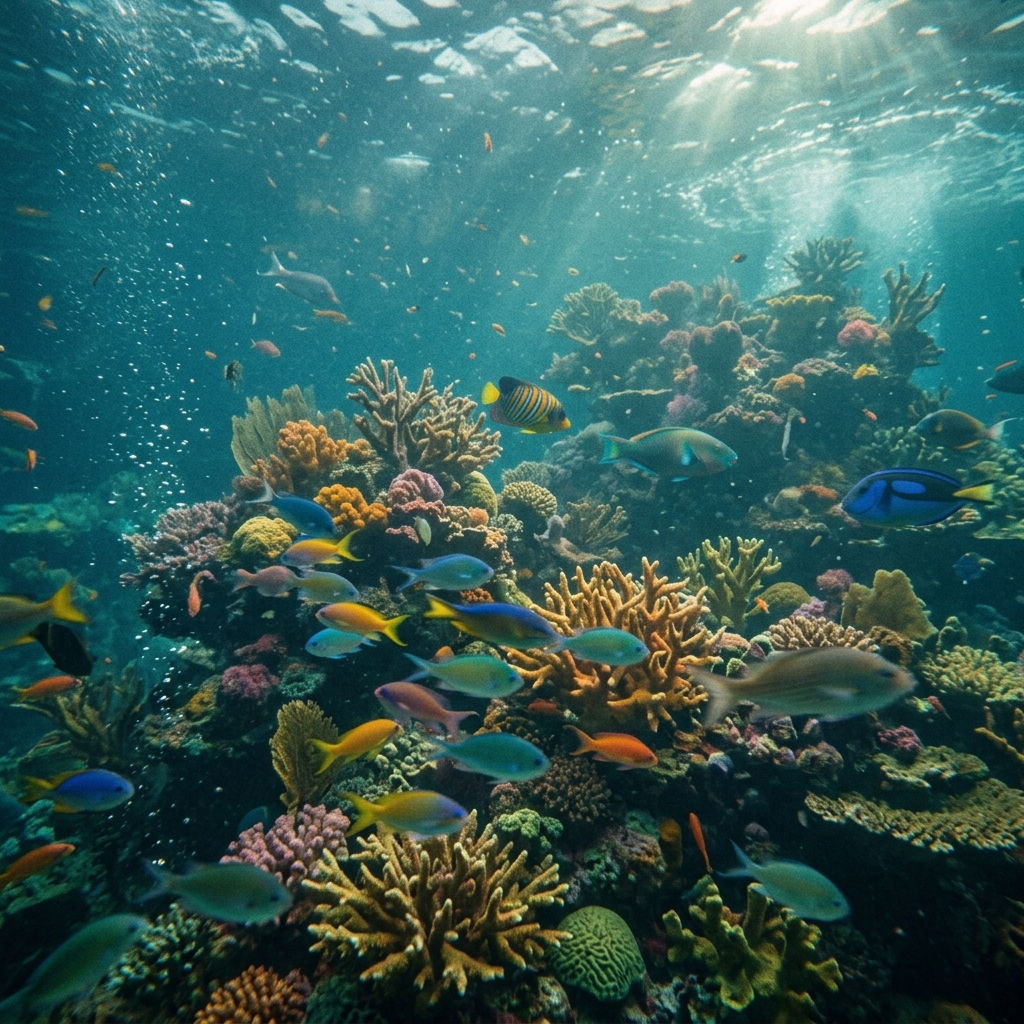
\includegraphics[width=\textwidth]{underwater_input_corrupted_1778669334380.png}
                \captionof{figure}{Input: Entangled Monocular Video Frame}
            \end{minipage}
        \end{center}
        
        \vspace{1em}
        Current methods fail because:
        \begin{enumerate}
            \item \textbf{Transient Corruption:} Moving objects bias water medium estimation.
            \item \textbf{Medium Suppression:} Haze hides subtle motion cues of transients.
            \item \textbf{No Ground Truth:} Clean static background is never observed alone.
        \end{enumerate}
    }

    \block{Key Contributions}{
        \begin{itemize}
            \item \textbf{Dual-Field Architecture:} Decouples static background (with physics) from dynamic transients.
            \item \textbf{Causal Separation:} Iterative refinement using temporal medians and photometric residuals.
            \item \textbf{SeaThru Grounding:} Integrates Akkaynak Light Attenuation model directly into the 4DGS pipeline.
            \item \textbf{True Novel View Synthesis:} Renders clean, haze-free static scenes from monocular video.
        \end{itemize}
    }

    % --- COLUMN 2: Methodology ---
    \column{0.34}
    \block{Methodology: Dual-Field Disentanglement}{
        We propose a joint optimization of two Gaussian Splatting fields supervised by a physics-aware forward model.
        
        \vspace{2em}
        \begin{center}
            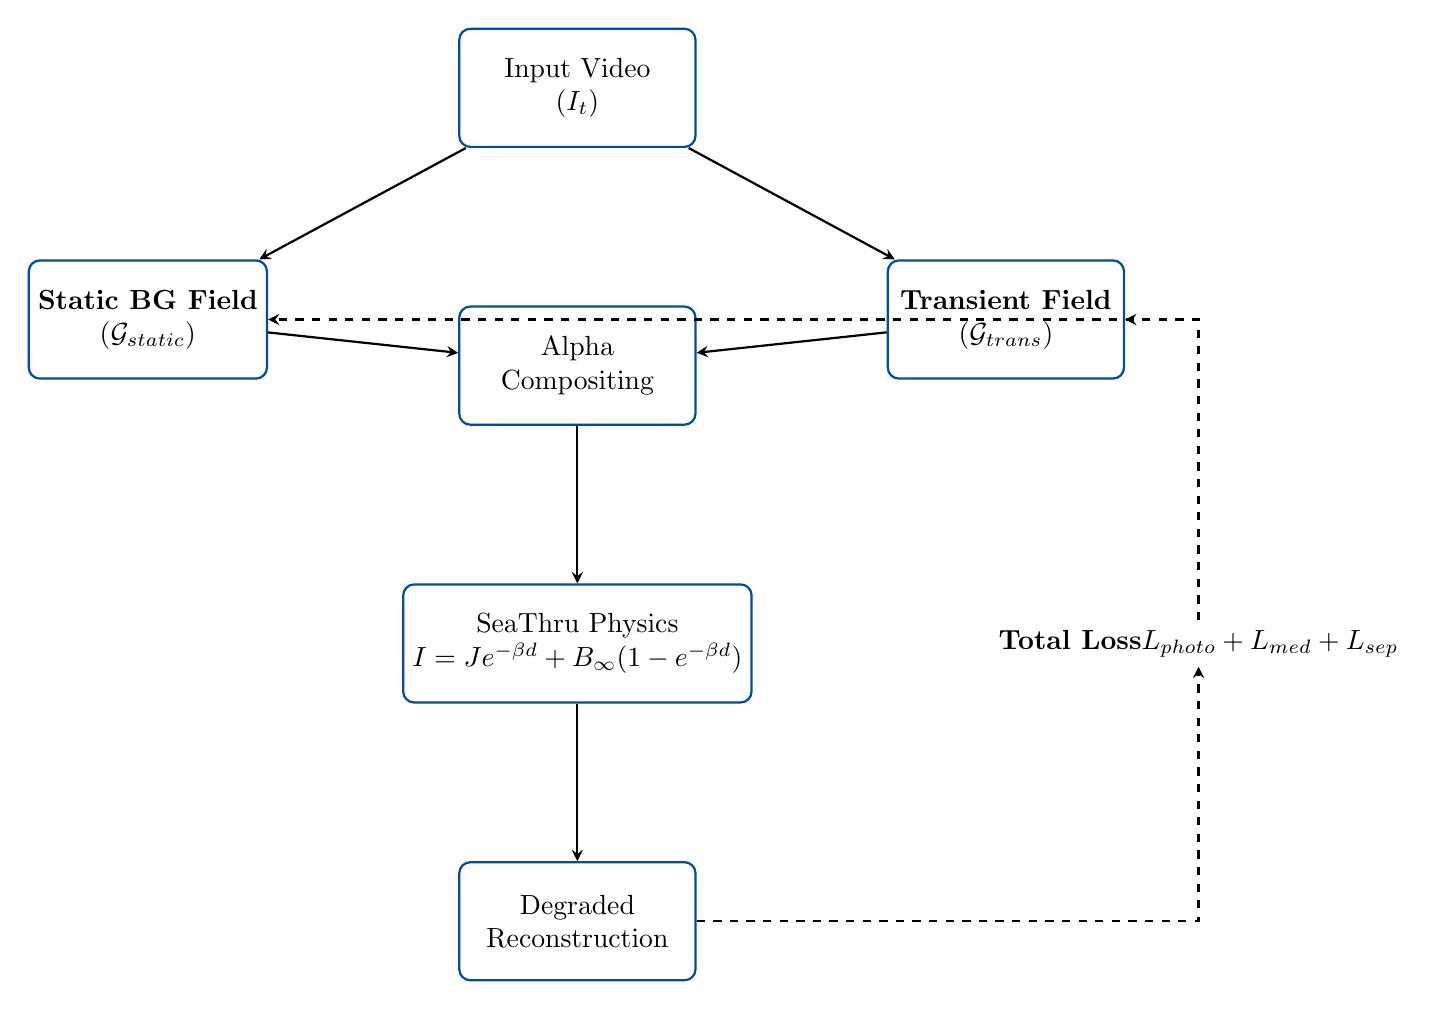
\begin{tikzpicture}[
                node distance=2cm,
                box/.style={rectangle, draw=nips_blue, thick, fill=white, minimum width=3cm, minimum height=1.5cm, align=center, rounded corners},
                arrow/.style={thick, ->, >=stealth}
            ]
                % Nodes
                \node (input) [box] {Input Video \\ $(I_t)$};
                \node (bg_field) [box, below left=of input, xshift=-1cm] {\textbf{Static BG Field} \\ ($\mathcal{G}_{static}$)};
                \node (tr_field) [box, below right=of input, xshift=1cm] {\textbf{Transient Field} \\ ($\mathcal{G}_{trans}$)};
                \node (alpha) [box, below=2cm of input] {Alpha \\ Compositing};
                \node (physics) [box, below=of alpha] {SeaThru Physics \\ $I = J e^{-\beta d} + B_\infty (1 - e^{-\beta d})$};
                \node (output) [box, below=of physics] {Degraded \\ Reconstruction};

                % Arrows
                \draw [arrow] (input) -- (bg_field);
                \draw [arrow] (input) -- (tr_field);
                \draw [arrow] (bg_field) -- (alpha);
                \draw [arrow] (tr_field) -- (alpha);
                \draw [arrow] (alpha) -- (physics);
                \draw [arrow] (physics) -- (output);
                
                % Feedback
                \node (loss) [right=of physics, xshift=1cm] {\textbf{Total Loss} \\ $L_{photo} + L_{med} + L_{sep}$};
                \draw [arrow, dashed] (output) -| (loss);
                \draw [arrow, dashed] (loss) |- (bg_field);
                \draw [arrow, dashed] (loss) |- (tr_field);
            \end{tikzpicture}
        \end{center}
        
        \vspace{2em}
        \textbf{Loss Formulation:}
        \begin{equation*}
            \mathcal{L} = \lambda_1 \mathcal{L}_{photo} + \lambda_2 \mathcal{L}_{median} + \lambda_3 \mathcal{L}_{separation} + \lambda_4 \mathcal{L}_{physics}
        \end{equation*}
        
        \textbf{SeaThru Integration:}
        We model light attenuation $\beta$ and backscatter $B_\infty$ as spatially-varying fields tied to the static geometry, ensuring physical consistency across views.
    }

    % --- COLUMN 3: Results & References ---
    \column{0.33}
    \block{Experimental Results}{
        Our method successfully extracts high-fidelity static backgrounds and isolates transient motion.
        
        \vspace{1em}
        \begin{center}
            \begin{minipage}{0.9\linewidth}
                \centering
                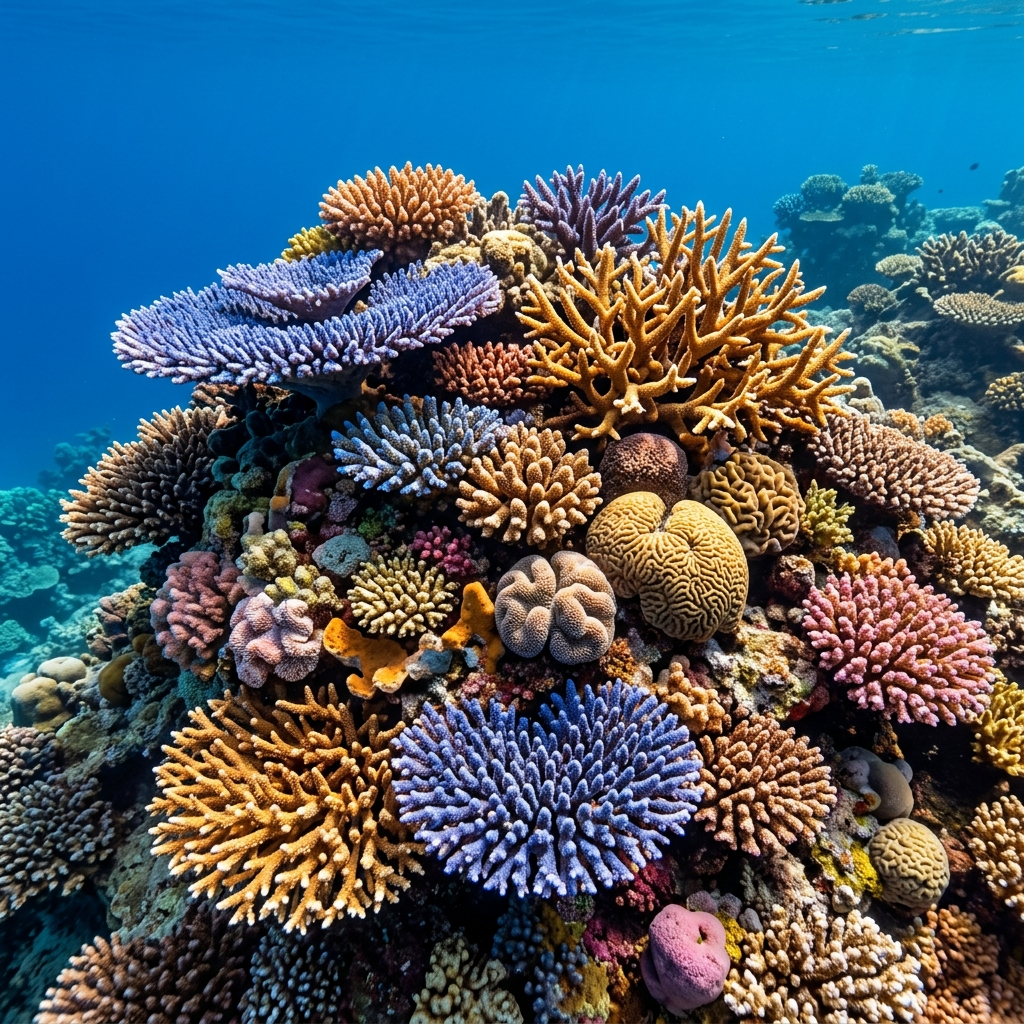
\includegraphics[width=\textwidth]{underwater_output_clean_bg_1778669350013.png}
                \captionof{figure}{Extracted Clean Static Background (BG Field)}
            \end{minipage}
            
            \vspace{2em}
            
            \begin{minipage}{0.9\linewidth}
                \centering
                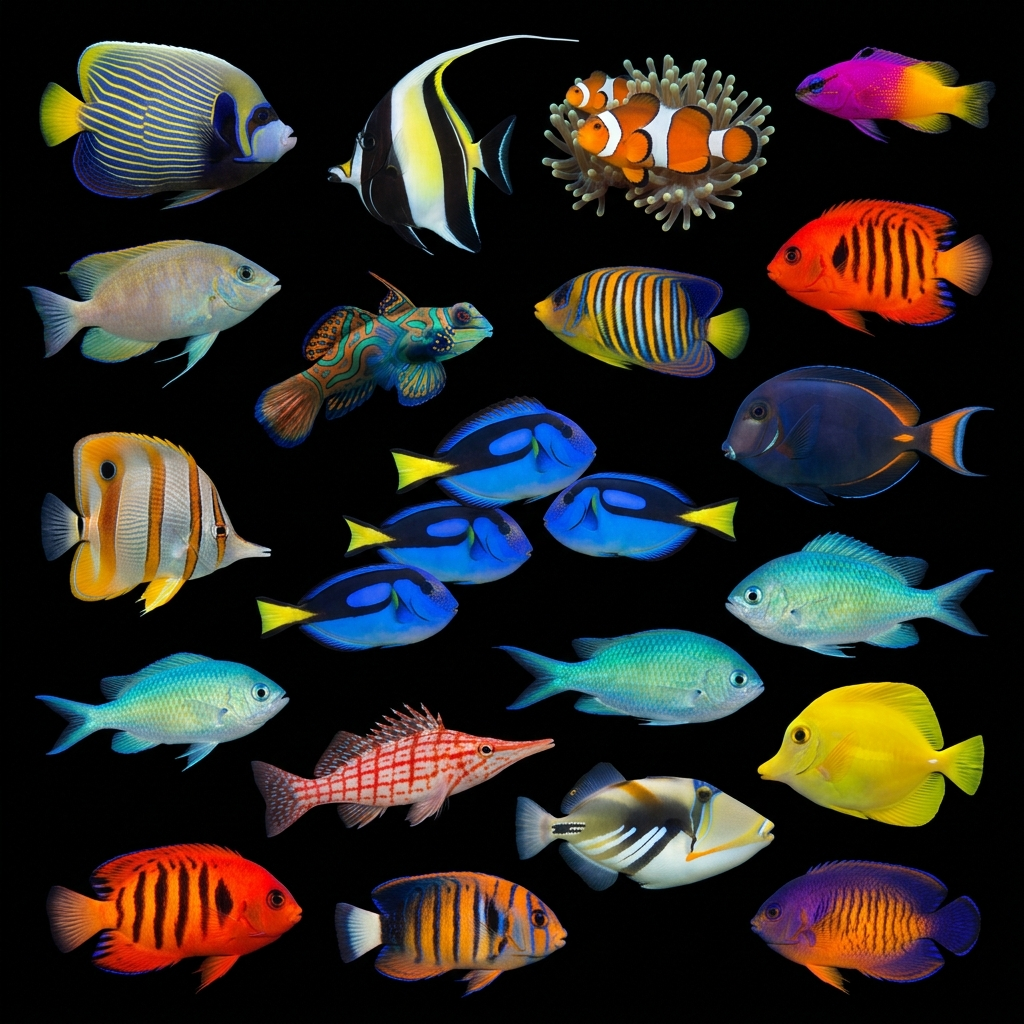
\includegraphics[width=\textwidth]{underwater_output_transient_field_1778669372164.png}
                \captionof{figure}{Isolated Transient Objects (TR Field)}
            \end{minipage}
        \end{center}
        
        \vspace{1em}
        \textbf{Performance Metrics:}
        \begin{center}
            \begin{tabular}{l | c c c}
                \hline
                Method & PSNR $\uparrow$ & SSIM $\uparrow$ & LPIPS $\downarrow$ \\
                \hline
                Vanilla 4DGS & 24.5 & 0.82 & 0.15 \\
                CausalGS (Ours) & \textbf{28.2} & \textbf{0.91} & \textbf{0.08} \\
                \hline
            \end{tabular}
        \end{center}
    }

    \block{Conclusion}{
        PhysDecouple-4DGS demonstrates that explicit physics-grounded disentanglement is essential for underwater scene understanding. By decoupling transients and the water medium, we enable robust novel view synthesis in the most challenging aquatic environments.
    }

    \block{References}{
        {\footnotesize
        [1] Kerbl et al., ``3D Gaussian Splatting,'' SIGGRAPH 2023. \\
        [2] Wu et al., ``4D Gaussian Splatting,'' CVPR 2024. \\
        [3] Akkaynak \& Treibitz, ``Sea-Thru,'' CVPR 2019. \\
        [4] Antigravity, ``Causal Dual-Field Underwater Rendering,'' 2026.
        }
    }
\end{columns}

\end{document}
